\chapter{Problem Statement and Solution Overview} \label{chap:ProblemAndSolution}
\begin{flushright}{\slshape    
   Science, my boy, is made up of mistakes, but they are mistakes
   which it is useful to make, because they lead little by little
   to the truth}. \\ \medskip --- \citeauthor{verne_journey:1957}
   \citetitle{verne_journey:1957} \citeyear{verne_journey:1957}
\end{flushright} 

\lettrine[lines=4]{\textcolor{purple}{B}}{ig} data applications are widely used in the industry and research fileds. Specialized   distributed frameworks are used to execute these applications on clusters of computers, very often made by cloud computing resources, like virtual machines and virtual storage. Apache Spark is probably the most popular big data processing framework. Spark organizes computations in directed acyclic graphs (DAG's) and its declarative API offers the capability to make transformations to datasets and return results to the client program, usually a standard Java, Python or Scala application. 

Spark starts executing a program by identifying jobs, delimited by the presence of actions in the code, and stages (within jobs), delimited by operations that require data to be shuffled (i.e., moved among executors), thus breaking locality. Indeed, Spark distinguishes
between narrow and wide transformations specifically for this purpose; the former do not shuffle data (e.g., map, filter, etc.), while the latter do (e.g., reduceByKey, etc.). Spark “identifies” all the operations that are to be executed, up to the first action, and
materializes them as a directed acyclic graph (DAG). The DAG is not the control-flow graph of the job’s code. It does not contain branches and loops since they were already resolved during the execution of the driver program. The DAG defines the execution order among stages, and defines the extent to which stages can be executed in parallel. For each job, Spark computes a DAG also called \textit{Parallel Execution Plan} (\plan) to maximize the parallelism while executing an application. In fact, a stage is, by definition, executed in parallel, and also different stages can be executed at the same time. For this reason, Spark materializes \plans as directed acyclic graphs of stages while the complete \model of an application is simply the sequence of the \plans of its jobs .A Spark application is usually composed by several jobs executed using a LIFO queue, therefore the \model of a Spark application is composed by the sequence of the \plans generated by the application jobs (an action corresponds to a job). In fact, Spark does not "compile" the code of the driver program to generate the application \model but it incrementally generates it as soon as an action is reached.

\section{Problem Statement}\label{sec:problem_statement}
Our goal is to support efficient execution of deadline-based QoS constrained multi-{\model} Spark applications, i.e. applications whose execution flow cannot be represented with a single \plan, and whose actual execution flow is only known at application execution runtime. In addition, the execution time is constrained by a user-defined deadline, that is the expected duration of the application.

The literature contains several works exploring adaptation capabilities, formal guarantees or response time estimation for Spark applications based on their \plan-based structure~\cite{dSpark, xsparkreport, Quattrocchi2018}, assuming that the \plan of the application does not change with respect to different data input or parameters. However, the \plan uniqueness assumption does not hold if conditional branches or loops are present in the control flow of the client program.

This is particularly relevant in Spark because of the possibility of evaluating
partial results through actions. In fact, these values can be used in the code as part of conditional expressions that can create branches in the control flow graph. In this cases the conditional branches govern the final structure of the \plan and also the operations that form a stage while loops influence the number of repetition of either transformations, stages or actions. 

Our solution is based on xSpark, a modified version of Apache Spark, developed at Politecnico di Milano~\cite{xsparkreport, Quattrocchi2018}, that has demonstrated the capability to execute deadline-constrained single-\plan applications by using resources more efficiently than  Spark would do in running the same applications. xSpark is able to use less resources than native Spark and can complete executions with less than 1\% error in terms of set deadlines.

Given all the above stated, in order to reach our objective of efficiently running deadline-based QoS constrained multi-\plan Spark applications, we need to positively answer to the following Research Questions:
\begin{enumerate}[\boldmath$RQ_1 $] 
	\item - [Effectiveness]:  Does our solution effectively control the execution of the Spark applications?
	\item - [Efficiency]:  To what extent can our solution improve the resource allocation capabilities of \cSpark, given it used a single, constant \plan?
\end{enumerate}
Most of the approaches in the literature (e.g., \cite{gibilisco2016stage,Sidhanta2016, dSpark, nfm}) use the execution graph to reason on the work to do, the degree of parallelism, the duration of tasks, and other application-specific characteristics. They also assume that the graph does not change since many of the conditional  branches and loops are hidden in the code (e.g., filter, map). As said, this is wrong when the code contains explicit loop and conditional statements.

For example, one can think of a simple two-job application. The first job retrieves some records from a data source (e.g., a file) and filters them according to a given criterion; the second job sorts them and returns the first $x$ records. To avoid problems, one may constrain the execution of the second job to the fact that the cardinality $c$ of filtered records, that is, the result produced by the first job, is greater than zero. The execution graph would then comprise two jobs $if c \geq 0$; it would only comprise the first job otherwise. This simple example shows how Spark can return partial results ($c$) through actions to the driver program and use these results to evaluate conditional (loop) expressions, and thus produce different execution graphs.

To overcome this problem, \cSpark and many solutions~\cite{Sidhanta2016, dSpark} exploit an initial profiling phase to retrieve the execution graph and collect some performance metrics. Back to the simple example sketched above, the initial profiling would simply return the execution graph implied by the data used to run the application. This single choice impacts the quality of obtained results and there is currently no means to adjust the graph with respect to the different data.
Even if one adopts a conservative approach and retrieves the execution graph that corresponds to the worst case (i.e., two jobs in the previous example), this would result in over-allocating resources and/or over-estimating execution times. If one adopted the best case (one job), too few resources and too short execution time would be foreseen.

\begin{figure}[htbp]
	\begin{small}
		\begin{verbatim}
		1  from pyspark import SparkContext
		2  def run(numIterations, threshold):
		3    sc = SparkContext('local','example')
		4  	 x = sc.textFile(...).map(...).groupBy(...)
		5     .map(...).aggregate(...)
		6    y = sc.textFile(...).map(...).groupBy(...)
		7     .map(...).aggregate(...)
		8    if x > threshold and y > threshold:
		9      for i in range(numIterations):
		10       z = sc.parallelize(...).map(...).sort(...).take(10)
		11   if x > y:
		12       w = sc.parallelize(...).map(...).filter(...).count()
		\end{verbatim}
	\end{small}
	\caption{Example Spark application with conditional branches and loops.}
	\label{fig:xdag2-code}
\end{figure}


The execution graph can also depend on user parameters or local variables and they must be considered in a sound analysis. For example, Figure~\ref{fig:xdag2-code} shows the code of an example application that takes two input parameters \textit{numIterations} and \textit{threshold}; its execution graph depends on both user parameters and input dataset. The first two \textit{aggregate} jobs\footnote{In Spark \textit{aggregateByKey} is a transformation while \textit{aggregate} is an action.} are always executed (line $4$ and $6$) and the results are assigned to variables $x$ and $y$, respectively. Line $8$ checks if both variables are greater than \textit{threshold}. If it is the case, a \textit{take} job (line $10$) is repeated \textit{numIterations} times (\verb#for# loop). Finally, if $x > y$ (line $11$) \textit{count} (line $12$) is executed. 

This simple code corresponds to four possible execution graphs (Figure~\ref{fig:xdag2}): i) the sequence of the two \textit{aggregate}s  (if the two conditional statements are both false) ii) the sequence of the two \textit{aggregate}s and \textit{take} repeated \textit{numIterations} times (if the first conditional statement is true and the second is not) iii) the sequence of the two \textit{aggregate}s and \textit{count} (if the second conditional statement is true but not the first), and iv) the concatenation of the two \textit{aggregate}s, \textit{take} repeated \textit{numIterations} times, and \textit{count} (if both conditional statements are true).

\begin{figure}[t]
	\centering
	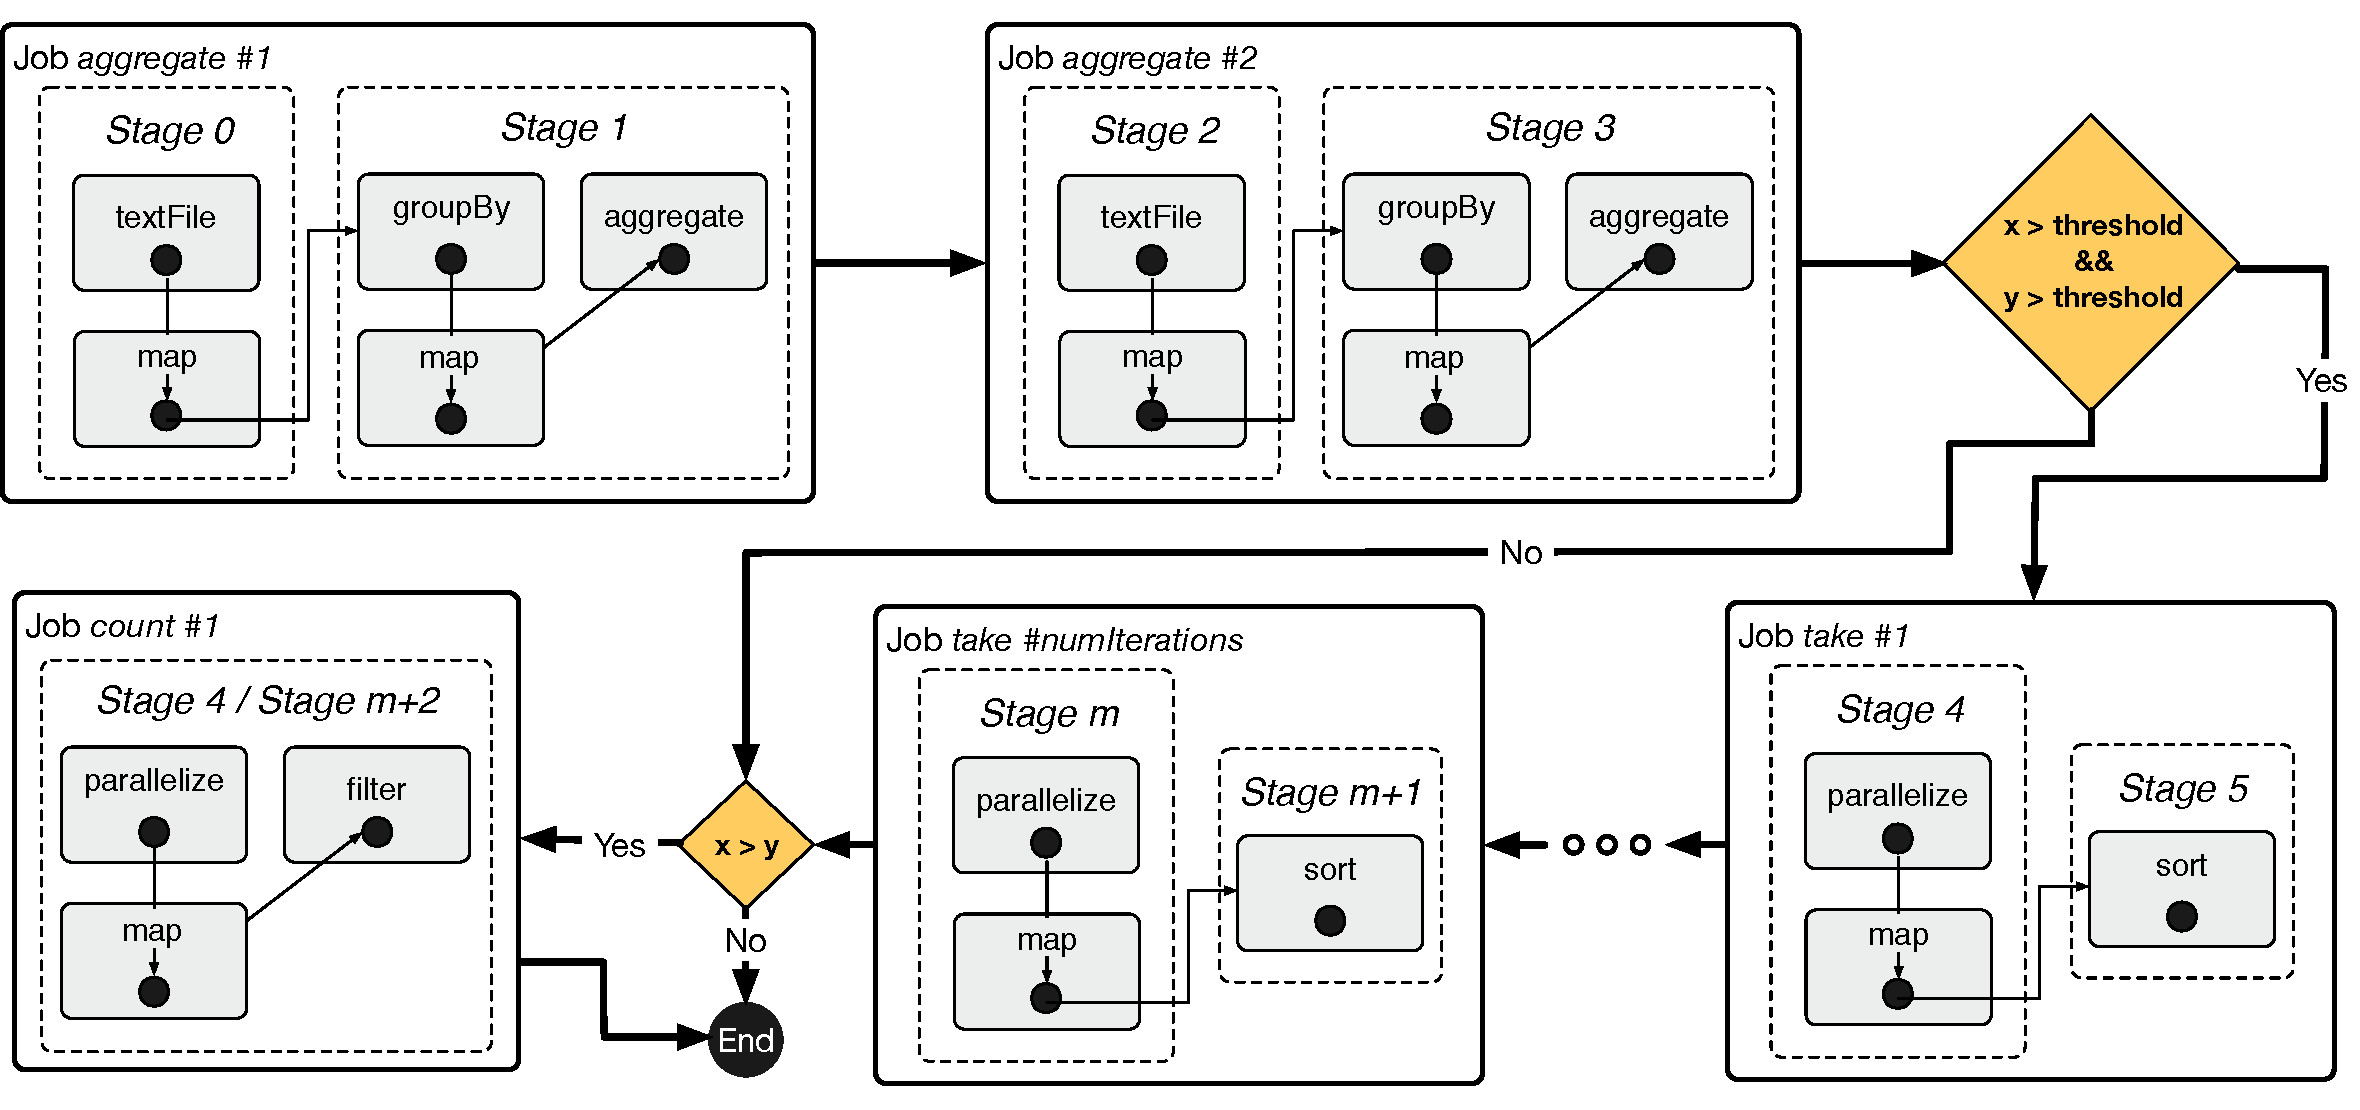
\includegraphics[width=1\columnwidth]{images/xdag2.pdf}
	\caption{The four  \plans of the application of Figure~\ref{fig:xdag2-code}.}
	\label{fig:xdag2}
\end{figure}

\section{Solution Overview}\label{sec:solution_overview}
This section contains a functional level description of the proposed solution, of its components and their interactions to make the solution work.

This thesis work presents \tool, a toolchain providing the capability to manage the efficient execution of deadline-based QoS constrained multi-\plan Spark applications. 

\tool is the result of the integration of \dSymb, a tool exploiting symbolic execution techniques to generate the path condition associated to each possible {\plan}s produced by different inputs and parameters, with (a modified version of) xSpark.
 Moreover, \tool generates a launcher with a synthesized dataset for each \plan and an artifact to retrieve the feasible {\plan}s given a set of symbolic variables  resolved to a value. Finally, we integrated this approach with xSpark, an extension of Spark that can control the duration of Spark applications according to specified deadlines through dynamic resource allocation. 
 
The evaluation shows that \approach is able to effectively extract all the DAGs generated by Spark applications and that xSpark reduces the number of deadline violation thanks to the presented integration.
In the remainder of this section we will go through a more detailed explanation of the solution's components and how they cooperate to provide the final result.

\subsection{\approach}\label{sec:symb}

In this section we describe \approach, \emph{Symbolic Execution-driven Extraction of Parallel Execution Plans}, an original combination of lightweight symbolic execution and search-based test generation that allows us to extract the \model of Spark applications. A \model  associates each control-flow path of the target application with the \plan generated by its execution, the relative profiling data, and the path condition that activates the path. 

\approach consists of four main phases: i) it relies on a lightweight symbolic execution of the driver program of the Spark application to derive a representative set of execution conditions of the control-flow paths in the program; ii) it exploits those execution conditions with a search-based test generation algorithm, to compute sample input datasets that make each path execute; iii) it executes the target application with those datasets as input, to profile the \plan generated by each path, and synthesize the \model accordingly; iv) it generates an artifact called \textit{GuardEvaluator} that returns the feasible \plans given a partial set of concrete values of the symbolic variables.
%In particular, for each  control-flow path analyzed during symbolic execution, the \model stores the execution conditions of the path, the Spark-DAGs of the jobs that Spark executes throughout the path, and the relevant execution-time data profiled during the execution. 
We exploit the information in the \model computed with \approach to extend \cSpark (see Section~\ref{sec:control}) with the ability of tuning its adaptation strategy according to the worst-case behaviour of the application. At runtime, our extended version of \cSpark exploits the \textit{GuardEvaluator} to refine the control policy by recomputing the worst-case estimation every time the current worst-case refers to a program path for which the execution condition stored in the \model becomes unsatisfiable.
%
Below, we describe each phase of \approach in detail.

\subsection{Lightweight Symbolic Execution}\label{sec:lightweight_symbolic_execution}
\approach relies on a lightweight symbolic execution of the driver program of the Spark application to identify the execution conditions of the feasible program paths of the driver program. To this end, \approach
models with unconstrained symbolic values the results of the parallel computation jobs issued in the driver program, 
% that correspond to the jobs defined in the driver program, 
thus abstracting from the details of those computations, and symbolically  analyzes the dependencies of the program paths on these symbolically modeled results.
%This simplifies the symbolic execution  working under the very conservative (though possibly imprecise) assumption that every distributed computation launched during the execution of the driver program may yield any possible result.  
\approach leaves for the subsequent test generation phase the burden of identifying concrete input datasets that make the parallel computation jobs encompassed in the driver program yield results that satisfy the path constraints identified during symbolic execution.

This section formalizes the lightweight symbolic execution algorithm of \approach for a simple imperative programming language in which all operations are either assignments of program variables or assume operations. The assignments are in the form \texttt{x := e}, where \texttt{x} is a program variable and \texttt{e} is an expression of values of program variables. The assume operations are in the form \texttt{assume(c)}, where \texttt{c} is a condition on the values of program variables, with the semantics that the program continues to execute only if the condition \texttt{c} evaluates to \emph{true}. 
A program in this language defines a transition system with a finite set of program locations $L \triangleq \{\ell_1, \ell_2, \dots, \ell_n\}$, a specified initial location $\ell_{init} \in L$, and a transition relation $T \triangleq \{t  \equiv \langle\ell, op \rightarrow \ell'\rangle\}$ that states the semantics of the program that can move from $\ell\in L$ to $\ell'\in L$ by executing a valid assignment or assume  operation $op$.

Two special classes of assignments, that is, assignments of the form \texttt{x := parallel\_op($\dots$)} and \texttt{x~:= aggregation\_op($\dots$)}, respectively, define parallel computations. 
The assignments \texttt{x := parallel\_op($\dots$)} assign the variable \texttt{x}
of the special type \emph{Dataset} to the result of the
expression \texttt{parallel\_op($\dots$)}, which in our context can refer to evaluating any of the parallel computation operations allowed in Spark (e.g., \texttt{map}, \texttt{filter}, \texttt{reduceByKey}).
The assignments \texttt{x~:= aggregation\_op($\dots$)} assign the variable \texttt{x}
to the result of a data aggregation operation, e.g., \texttt{count}, \texttt{collect}, etc, evaluated against a dataset computed in parallel fashion. 
%Our symbolic execution algorithm does not interpret the possible input parameters of these operations, such as for example the parameters in the the expression \texttt{data.map($\lambda$)} that receives and input dataset \texttt{data} and a function \code{$\lambda$} to execute in parallel fashion. 

Figure~\ref{fig:symbex} defines the symbolic execution algorithm of \approach. We denote the symbolic states computed during the analysis with $s \equiv \langle \ell, vv, pc\rangle$, being $\ell$ the program location to which this symbolic state refers, $vv$ the set of program variables assigned so far, and $pc$ (the path condition) the path constraint due to the assume operations traversed so far. The algorithm starts from the initial state $s\_{init} \equiv \langle \ell_{init}, \emptyset, true\rangle$ (no variable assigned, unconstrained path), and unfolds the transitions of each program path by recursively executing the atomic step $s'\gets SE(s, t)$ of Figure~\ref{fig:symbex}, where $s'$ is the state reached from $s$ when executing the transition $t$. 


\begin{figure*}
	\newcommand{\code}[1]{ \text{\texttt{#1}}}
	\tiny
	\[SE(s\equiv\langle \ell, vv, pc\rangle, t\equiv\langle \ell, op \rightarrow \ell'\rangle) \triangleq 
	\begin{cases}
	
	\langle \ell', vv[\code{x} \gets \llbracket \code{e}\rrbracket_{vv})], pc\rangle
	& \text{ if } 
	op \equiv \code{x := e}\\
	
	\langle \ell', vv, pc \wedge \llbracket \code{c}\rrbracket_{vv}\rangle
	& \text{ if } 
	op \equiv \code{assume(c)}\\
	
	\langle \ell', vv[x \gets \delta], pc\rangle
	& \text{ if } 
	op \equiv \code{x := \textit{parallel\_op}($\dots$)} \text{ e.g. }
	\begin{cases}
	\code{sparkCtx.textFile($\dots$)}\\ % \code{sparkCtx.parallelize($\dots$)}\\
	\code{data.map($\lambda$)}\\ \code{data.filter(\textit{$\lambda$}))}\\ \code{data.reduceByKey(\textit{$\lambda$})}\\ \code{data.groupBy($\lambda$)}\\ \code{data.flatMap($\lambda$)}\\ \code{data.aggregateByKey($\lambda$)}\\ \code{data.cartesian($\lambda$)}\\ 
	\dots
	\end{cases}\\
	
	
	\langle \ell', vv[x \gets \alpha_\ell], pc\rangle
	& \text{ if } 
	op \equiv \code{x := \textit{aggregate\_op}($\dots$)}  \text{ e.g. }
	\begin{cases}
	\code{data.count()}\\ \code{data.collect()}\\ \code{data.take(n)}\\ \dots
	\end{cases}\\
	
	\end{cases}
	\]
	
	\caption{Symbolic execution algorithm of \approach.}
	\label{fig:symbex}
	\normalsize
\end{figure*}

Figure~\ref{fig:symbex} specifies the algorithm as a list of four cases. The first two cases describe the classic symbolic execution algorithm that handles 
\begin{inparaenum}[(i)]
	\item the assignment operations  \texttt{x := e} by setting the variable \texttt{x} to the value of expression \texttt{e} in the current state %($x \gets \llbracket e\rrbracket_{vv}$), and 
	\item the assume operations \texttt{assume(c)} by conjoining the current path condition with the value of condition \texttt{c} in the current state ($pc \wedge \llbracket \texttt{c}\rrbracket_{vv}$). 
	%
	The last two cases in Figure~\ref{fig:symbex} define the abstract modeling of the assignments that involve parallel operations:  
	\item the assignments \texttt{x~:= parallel\_op($\dots$)} result in setting the variable \texttt{x} to the unique symbolic value $\delta$, which we use to symbolically model every dataset accessed and computed in the program; \item the assignments \texttt{x := aggregation\_op($\dots$)} result in setting the variable \texttt{x} to a new unconstrained symbolic value $\alpha_\ell$ that model the result of the aggregation operator called at the program location $\ell$.  (For simplicity the figure omits the further incremental index that we use to symbolically model the results of subsequent assignments at a location that is traversed multiple times in the same program path.)
\end{inparaenum}

The right part of Figure~\ref{fig:symbex} exemplifies a set of both \texttt{parallel\_op} and \texttt{aggregation\_op} operations. These examples include only a subset of the available Spark operations. Beyond these examples, with reference to the RDD Programming Guide~\cite{RDDGuide:online:2019}, the  \texttt{parallel\_op} operations of Figure~\ref{fig:symbex} encompass the complete list of \emph{transformation} and \emph{shuffle} operations, while the  \texttt{aggregation\_op} operations encompass all \emph{action} operations. 

An important remark about the algorithm is that the conditions of the assume operations defined in the driver program cannot explicitly predicate on the internal state of variables of type \emph{Dataset}. In fact, although the variables of type \emph{Dataset} undergo parallel computations, the data produced with these computations may propagate in the driver program only indirectly, as the result of invoking some \texttt{x := aggregation\_op(...)} operation. Thus, the assume operations in the driver program may predicate only on variables assigned as \texttt{x := e} and \texttt{x := aggregation\_op(...)}. 
This guarantees that the symbolic value $\delta$ that models the assignments \texttt{x~:= parallel\_op(...)} never appears in a path condition, which is the reason why we can embrace the simplification of using this single symbolic value to abstractly model all the datasets that the target driver program may manipulate. 

\approach uses the algorithm Figure~\ref{fig:symbex} to symbolically analyze the paths of the target driver program, and returns the path condition computed for each path. As usual in symbolic execution, we use a constraint solver to check if any path condition formula becomes unsatisfiable at some point of the analysis, and dismiss the analysis of the program paths with unsatisfiable path conditions.  Our current \approach prototype implements the algorithm described in this section on top of the symbolic executor JBSE~\cite{braione:jbse:fse:2016} that relies on the constraint solver Z3~\cite{demoura:z3:tacas:2008}.

For example, for the Spark application in Figure~\ref{fig:xdag2-code}, when analyzing the paths of the driver program that do not enter the loop at line~9, 
\ (let $\alpha_5$ and $\alpha_7$ be the symbols that represent the results of the \texttt{aggregate} actions at line~5 and line~7, respectively, and $thresh$ and $iters$ the symbols that represent the input values of parameters \texttt{threshold} and \texttt{numIterations}, respectively) \approach computes the path conditions:
\begin{itemize} 
	\item \(\alpha_5 \le thresh \wedge \alpha_5 > \alpha_7\);
	\item \(\alpha_5 \le thresh \wedge \alpha_5 \le \alpha_7\);
	\item \(\alpha_5 > thresh \wedge \alpha_7 \le thresh \wedge \alpha_5 > \alpha_7\);
	\item \(\alpha_5 > thresh \wedge \alpha_7 > thresh \wedge iters \le 0 \wedge  \alpha_5 > \alpha_7\);
	\item \(\alpha_5 > thresh \wedge \alpha_7 > thresh \wedge iters \le 0 \wedge  \alpha_5 \le \alpha_7\);
	
\end{itemize}
%
while it identifies the unsatisfiable path condition \(\alpha_5 > thresh \wedge \alpha_7 \le thresh \wedge \alpha_5 \le \alpha_7\).

For programs with loops, like the one in the figure, \approach bounds the iterations of the loops to an user-defined maximum value, thus guaranteeing to have to symbolically analyze a finite amount of paths. 

\subsection{Search-Based Test Generation}
\approach exploits the path conditions identified with symbolic execution as above, to generate test cases (a test case for each path condition) comprised of input values and input datasets that make the target Spark application concretely execute  the  paths of the driver program that correspond to the path conditions. The goal is to use these test cases in the next phase of \approach,  to profile the behavior of the \plan generated by the execution each path of the driver program.

To generate a test case for a given path condition,  \approach incrementally explores the space of the possible test cases in search-based fashion, steering the search with a fitness function that quantifies the extent to which each incrementally considered test case is close to (or far from) satisfying the path condition at hand. Below, we first describe the \approach search algorithm in detail, and then explain the 
test execution sandbox that the algorithm uses to speed up the execution of the test cases. 

\subsubsection{Search Algorithm}
The \approach search algorithm generates test cases that call the target application with 
the inputs (both the input parameters and the input datasets) assigned to concrete values (both concrete values of the parameters and and concrete datasets). 
The algorithm samples the possible values of the inputs in the style of \emph{genetic algorithms}. It starts with generating a \emph{population} of test cases comprised of randomly picked inputs, and then \emph{evolves} from the initial population, by incrementally generating a series of next-generation populations, each obtained 
by manipulating the test cases in the previous-generation population with \emph{mutation} and \emph{crossover} operators. 
Mutation operators generate new test cases by randomly modifying some inputs of a test case of the previous-generation population. The crossover operators generate new test cases as the children of some pair of test cases of the previous-generation population, by conjoining inputs taken from either test case of the pair. 

The \approach fitness function quantifies the goodness of each generated test case with respect to the goal of satisfying a path condition, one of those identified in the previous phase, yielding a value that we interpret as the distance of the current test case from a satisfying test case: If the fitness function yields a distance of 0, the current test case is indeed a satisfying test case, and the search algorithm returns it as result; Otherwise, the fitness function yields a value greater than zero that the search algorithm exploits to comparatively order the test cases of the current population.  The search algorithm proceeds with probabilistically favouring the application of mutation and crossover operators to 
test cases with lower distance from the goal, thus increasing the chances to eventually converge to a satisfying test case. 

In detail, \approach computes the fitness of a test case with respect to a path condition as follows. First, it executes the test case, and collects the results of the Spark aggregation actions that the driver program executes thereby. Next, it evaluates the path condition for the valuation of the symbolic values induced by the execution of the test case, that is, by assigning the symbolic values that model input parameters to the concrete values set in the test case, and the symbolic values that model results of aggregation actions (the $\alpha_\ell$ symbols of Figure~\ref{fig:symbex}) to the corresponding results collected while executing the test case. If the test case does not execute an aggregation action referred in the path condition, we assign the corresponding symbol to the special value $Undef$. Then, if there are no $Undef$ symbols, and if the path condition evaluates to $true$ for the concrete assignment induced by the test case, then the fitness is zero: indeed the test case satisfies the path condition. Otherwise, the fitness is the positive value yielded by the following formula (let $t$ be the test case, and $pc$ be the path condition):
%
\[fitness(t, pc\equiv c_1\wedge c_2\wedge\dots\wedge c_n) = \sum_{i=1}^{n} distance(t, c_i)\]

\noindent where $c_i$ are the atomic conditionals in the path condition $pc$, and the function $distance$ that appears in the summation recursively computes the distance of each atomic conditional from being satisfied. In turn, the function $distance$ is defined as follows (let $c \equiv o_1 \bowtie o_2$ be a conditional, where $\bowtie$ is a comparison operator and $o_1$, $o_2$ are operands, either literals or symbolic expressions): 

\[distance(t, c) \triangleq 
\begin{cases}
0, \text{~~~~if } t(o_1) \bowtie t(o_2)= true\\
1, \text{~~~~if } t(o_1)= \text{Undef } \vee t(o_2)= \text{Undef}\\
1-\dfrac{1}{1 + |t(o_1)-t(o_2)| + \epsilon},  \text{~~~~otherwise}
\end{cases}\]

\noindent where $t(o_1)$ and $t(o_2)$ are the values of the operands $o_1$ and $o_2$, respectively, for the concrete assignments set in the test case $t$,  $t(o_1)$ and $t(o_2)$ are set to $Undef$ if they depend on any symbol assigned to $Undef$ after executing the test case, and $\epsilon$ is an arbitrary small number.

We make the following remarks about the \approach fitness function. Function $distance$ yields always a value in the interval [0, 1], and thus the overall $fitness$ ranges in the interval [0, n] for a path condition with $n$ atomic conditionals. Function $distance$ yields zero (first case in the formula) for satisfied conditionals, and thus the overall $fitness$ is zero only for a test case that satisfies all conjuncts, that is, a satisfying test case, as expected.  Function $distance$ yields the maximum value 1 (second case in the formula) for conjuncts that refer to any symbol assigned to $Undef$, and thus the overall $fitness$ is never zero if it depends on any symbol assigned to $Undef$, as expected. Function $distance$ yields values increasingly closer to zero (third case in the formula) if the operands of the referred conditional evaluate to increasingly mutually-closer values, meaning that the corresponding test cases are missing the satisfaction of the conditional for increasingly smaller amounts. Thus, the overall $fitness$ is  increasingly closer to zero, the higher the number of satisfied or close-to-be-satisfied conditionals, as expected.

%Come funzione di fitness usiamo la path condititon di ogni path, e quindi la soluzione ottima e' un insieme di dataset popolati con dati che, quando eseguiti dal driver program, portano ad eseguire il path identificato dalla path condition. 


\subsubsection{Test Execution Sandbox}
Each fitness evaluation issued in the above search algorithm requires, at least in principle,  the execution of the parallel application under test, which can quickly become computationally infeasible in consideration of the many test cases that the algorithm generates during the search. To address this issue, the \approach search algorithm executes the test cases in a test execution sandbox that specializes the RDD-typed datasets of the target Spark application as a custom type of datasets that we call \emph{sparse diversity data (\sparsedata) datasets}. 

A \sparsedata dataset  synthetically represents a RDD object with many data points that hold the same value. In \sparsedata format, a dataset is modelled as a list of data blocks, each with two attributes, namely, \texttt{size} and \texttt{value}: A data block with \texttt{size} equal to $s$ and \texttt{value} equal to $v$ 
stands for a set of $s$ data points, all with the same value $v$.  \approach uses the \sparsedata format to model datasets in which the amount of distinct values is significantly much smaller than the overall amount of values in the dataset. For example, a dataset with $20^9$ data points in which half of the data points have value 100 and the other half -100 can be very concisely represented with a \sparsedata dataset with two data blocks, both with \texttt{size} equal to $10^9$, and \texttt{value} equal to 100 and -100, respectively. 

The test execution sandbox recasts the computation of the parallel operations allowed for the RDD objects (e.g., operations like \texttt{map}, \texttt{filter}, \texttt{reduceByKey}, etc.) to sequencial operations executed against the data blocks in the \sparsedata objects. For example, a  \texttt{map($\lambda$)} transformation executed on a \sparsedata dataset $D$ with data blocks $[b_1, b_2, ..., b_n]$ yields a new \sparsedata dataset $D'$ with data blocks $[b'_1, b'_2, ..., b'_n]$  such that, for all $i=1..n$,  $b'_i.size := b_i.size$ and $b'_i.value := \lambda(b_i.value)$.
Similarly, a  \texttt{filter($\lambda$)} transformation on $D$ 
yields $D''$ with the subset of data blocks of $D$ that satisfy the condition $\lambda(b_i)$. Yet, a \texttt{count()} action on $D$ yields the value $\sum^i b_i.size$ as result. Our \sparsedata objects handle all transformations and actions defined in the RDD Programming Guide~\cite{RDDGuide:online:2019}. 


The crossover and mutation operators of the \approach search algorithm manipulate the input \sparsedata datasets of the target application by modifying, adding and removing data blocks (mutation operators) or combining the data blocks from the \sparsedata datasets in the parent test cases (crossover operator). 
Our current \approach prototype implements the search algorithm described in this section based on the SUSHI test generation framework~\cite{braione:combining:issta:2017, braione:sushi:icse:2018}. SUSHI converts the path conditions generated with JBSE in fitness functions as the ones described in this section, and adapts the test genetic search procedure of the tool EvoSuite~\cite{fraser:evosuite:tse:2013} to use these fitness functions. 

For example, with reference to a path condition computed for the Spark application in Figure~\ref{fig:xdag2-code}, e.g., one of those reported in the previous section, \approach may compute a test case resembling like the following one
\begin{verbatim}
Test:
1  threshold = 152;
2  numIterations = 0;
3  D1 = new SDD(size = 1000000, value = 721);
4  D2 = new SDD(size = 3000000, value = 814);
5  setInputTextFile(..., D1);
6  setInputTextFile(..., D2);
7  run(numIterations, threshold);
\end{verbatim}
that sets the input parameters \texttt{threshold}  and \texttt{numIterations} to concrete values (lines~1--2), builds two SDD datasets, both with a single data block (lines~3--4), sets these datasets as the input files that the application will read as input (lines~5--6), and executes the application with these inputs. 

\[a = \lceil b + c\rceil\]

\subsection{Synthesis of the \model}

\approach uses the test cases generated with the search algorithm, to execute the target Spark application, and profile the \plan generated by the execution of each path of the driver program. In this phase, \approach replaces the \sparsedata datasets that appear in the test cases yielded by the search algorithm with proper RDD datasets comprised of the same amount of data. It executes the test cases against the target application in fully parallel fashion. While executing each test case, \approach stores the \plan that the Spark engine produces before starting each parallel execution job, and monitors the parallel execution of the jobs to collects the timing data that are relevant for  the control policy. 

\approach builds the \model model as a set of triples \[\langle pc \rightarrow \plans, times\rangle\] where each triple represents the sequence of \plans  and the timing data --- $times$ --- associated with the execution of the test case that corresponds to the path condition $pc$. 

Together with the \model, \approach produces an an artifact that we call \textit{GuardEvaluator} that takes as input partial set of concrete values of the symbolic variables, evaluates the path conditions of  triples in the \model against these values, identifies which path conditions evaluate to $false$ for these values, and  
returns as output the subset of the \model with only the triples with non-falsified path conditions. In the control policy that we define in the next section, we invoke the guard evaluator at runtime, feeding it with the concrete values of the input parameters and incrementally with the concrete values of the executed actions, to stay tuned on the program paths that are possibly reachable at every intermediate execution state. 


\approach addresses the possible incompleteness of either its symbolic execution and search phase as follows. As we already commented above, in the symbolic execution phase, \approach analyzes the loops in the program up to a finite (user-configured) amount of iterations, and the analysis may thus produce incomplete results if it indeed happens to dismiss some program path (if any) that iterates any loop more than that amount. In this case, \approach tracks the path conditions $\hat{pc}$ that correspond to the interrupted prefix of the non-analyzed paths, and stores these path conditions in the \model as special triples with missing data \(\langle \hat{pc} \rightarrow \emptyset, -\rangle\).  Similarly, if the search algorithm fails to converge to the optimal solution for some path condition $\tilde{pc}$, \approach stores corresponding triples with missing data \(\langle \tilde{pc} \rightarrow \emptyset, -\rangle\). These special triples in the \model allow the control policy described in the next section to anticipate when an un-profiled path is going to be executed at runtime, and take decisions to mitigate the impact of these unforeseen situations. 


\subsection{xSpark$_{\text{\textit{\textbf{SEEPEP}}}}$}
This section describes how \dSymb integrates within \cSpark: the resulting tool-chain is called \tool. \dSymb produces the 
path conditions associated with the different \plans of the application, a set of test cases for each \plan for profiling, and a \textit{GuardEvaluator} to allow \cSpark to select the most appropriate \plan at runtime. At each execution step, \textit{GuardEvaluator} always returns the \plans whose associated path conditions still hold true. 


\begin{figure}[tbhp]
	\centering
	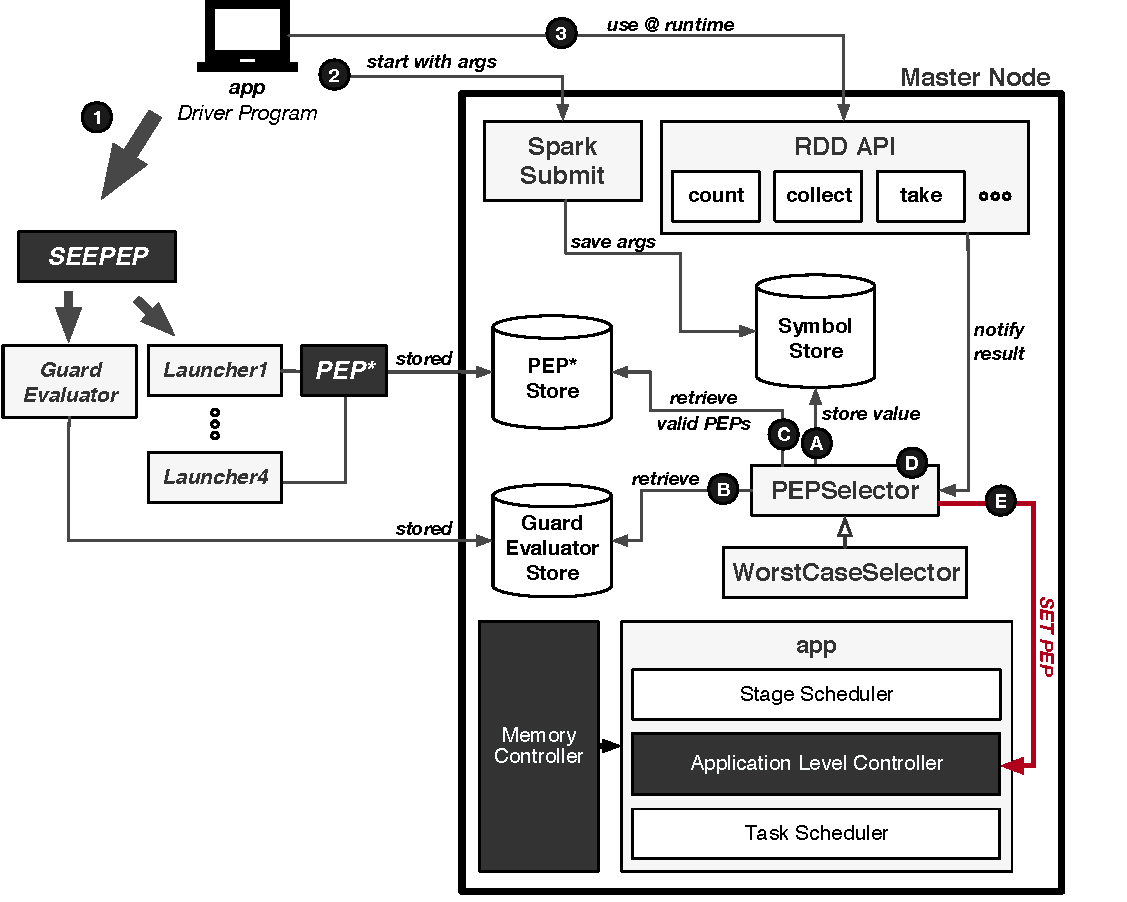
\includegraphics[width=\columnwidth]{images/xsparksymb}
	\caption{\tool}
	\label{fig:xsparkdagsymb}
\end{figure}

Figure~\ref{fig:xsparkdagsymb} shows the main elements of the tool-chain and exemplifies it on profiling and controlling the example application of Figure~\ref{fig:xdag2} ---\textit{app}, hereafter. As first step, \dSymb generates the $4$ ($n$, in general) launchers, which activate the four ($n$) \plans of the program, and an application specific \textit{GuardEvaluator}. 

The new toolchain associates each \plan to its path condition, it uses the generated launchers to obtain the profiling data of each \plan and synthesize the \model for the application that is then stored in the master node in component \textit{PEP* Store}. Finally the generated \textit{GuardEvaluator}, which implements a common interface to be dynamically instantiated and used without a static import in the source code of \cSpark, is also stored in the master node (component \textit{GuardEvaluator Store}).

After this phase, $app$ can be executed and controlled by \cSpark. 
Since the application parameters can be part of a path condition as symbols, we modified component \textit{SparkSubmit} to store their values. A symbol is identified by application name, action name, code line in the driver program, and a counter to take multiple executions into account  (i.e., loops or recursive functions). 

At runtime, everytime an action is executed, that is, a result is computed and returned to the driver program, our modified version of the  \textit{RDD API} notifies component \textit{PEPSelector} that a new result is available. This component is in charge of selecting the \plan and its profiling data then used by \textit{Application Level Controller} to compute the local deadlines for the next stages and thus to provision resources. \textit{PEPSelector} saves computed results into component \textit{Symbol Store}, retrieves an instance of the dedicated \textit{GuardEvaluator}, and feeds it with all the symbols resolved 
by the aforementioned results. \textit{GuardEvaluator} returns the list of \plan whose path conditions still hold.

This means, for example, that at the beginning of the execution of function \textit{run} of $app$, four \plans are valid since neither $x$ nor $y$ have been resolved to a value. The job at line $4$ produces the value of $x$ and if the value is less than or equal to $threshold$,  the if statement of line $8$ is not evaluated. Therefore, even if the value of $y$ is still unknown, \textit{GuardEvaluator} only returns two \plans, that is, the only two \plans whose path conditions still hold: it excludes all the path conditions that depends on the expression $x > threshold$). This way, since the \plan is updated constantly, \cSpark becomes aware of what has been actually done, and can use this information to refine resource provisioning.  

Note that \textit{PEPSelector} receives all the valid \plans and computes the next \plan to use. This selection can be customized by the user. Currently, we always select the worst-case \plan, that is, the \plan with the greatest number of remaining stages to be conservative and minimize deadline violations. If one wanted to optimize different performance indicators (e.g., deadlines are not strict and used resources must be minimized), the selection could privilege a \plan that corresponds to an average case instead of the worst one.